\documentclass[xcolor=table,final]{beamer} %,handout
\usepackage{etex}

\usepackage{amsfonts,amssymb}
\usepackage{url}
\usepackage{physics}
%% \usepackage{hyperref}

\usepackage[T2A]{fontenc}
\usepackage[utf8]{inputenc}
\usepackage[english]{babel}
\usepackage[linesnumbered,vlined]{algorithm2e}
\usepackage{booktabs}
\usepackage{fancybox}
\usepackage{blockmatrgraph}

\usepackage{tikz}
\usetikzlibrary{matrix,shadows,arrows,shapes,patterns,trees}
\usepackage{dirtree}

\usepackage{ulem}

\newcommand{\PageRank}{\texttt{PageRank}\xspace}

\newcommand{\Bsof}{\texttt{BSOF}\xspace}
\newcommand{\Bstri}{\texttt{BSTRI}\xspace}
\newcommand{\Bsoftri}{\texttt{BSOFTRI}\xspace}
\newcommand{\Bsoi}{\texttt{BSOI}\xspace}
\newcommand{\Gemm}{\texttt{DGEMM}\xspace}
\newcommand{\Trmm}{\texttt{DTRMM}\xspace}
\newcommand{\Trsm}{\texttt{DTRSM}\xspace}
\newcommand{\Lacpy}{\texttt{DLACPY}\xspace}
\newcommand{\Trtri}{\texttt{DTRTRI}\xspace}
\newcommand{\Geqrf}{\texttt{DGEQRF}\xspace}
\newcommand{\Orgqr}{\texttt{DORGQR}\xspace}
\newcommand{\Ormqr}{\texttt{DORMQR}\xspace}
\newcommand{\Ilaenv}{\texttt{ILAENV}\xspace}

\mode<presentation>{
  \hypersetup{pdfpagemode=FullScreen}
  
  %% \usetheme{Berkeley}
  %% \usecolortheme{crane}%{seagull}
  %% \usetheme{AnnArbor}
  \usecolortheme{rose}

  \setbeamercovered{transparent}
}

\mode<handout>{
  \useinnertheme{default}
  \useoutertheme{infolines}
  \usecolortheme{default}
  \usefonttheme{professionalfonts}

  \usepackage{pgfpages}
  \pgfpagesuselayout{2 on 1}[a4paper,border shrink=4mm]

  \setbeamercolor{structure}{fg=black}
  \setbeamerfont{structure}{series=\bfseries} 
}

\title[PageRank and Kempe-McSherry]{%
  Applying Orthogonal/Power Iterations to Big Graph Mining : \PageRank and Kempe-McSherry Algorithms}
\subject{Big Graph Mining}

\author[S.\,Gogolenko]{
  Sergiy Gogolenko %\inst{1} 
}

\institute[DonNTU]{%
  
\includegraphics[height=2cm]{./figs/logo/donntu-logo.png}%Donetsk National Technical University
  \hspace*{0.75cm}~%
  
\includegraphics[height=2cm]{./figs/logo/ucu-logo.png}%University of California, Davis
}
%% \titlegraphic{
\includegraphics[width=4cm]{./figs/logo/ucdavis-logo.png}}

\date[Lviv 2016] {%
  Ukrainian Catholic University, Lviv \\%
  \footnotesize{2016, May 23}
}


\pgfdeclareimage[height=1.2cm]{university-logo}{./figs/logo/ucdavis-logo.png}

\begin{document}

\frame[plain]{\titlepage}

\begin{frame}{Outline}%[pausesections]{Outline}
  \tableofcontents
\end{frame}

\section{\PageRank}

% %% \subsection{Problem formulation}

% \begin{frame}{Problem formulation}
%   \begin{definition}[$p$-cyclic matrix]
%     \begin{equation} \label{eq:matr_A}
%       H =
%       \begin{bmatrix}
%         A_1 &    &    &  & B_p   \\
%         B_1 & A_2 &    &  &  \\
%         & B_2 & A_3 &  &     \\
%         &        & \ddots & \ddots &         \\
%         &     &          & B_{p-1} & A_p
%       \end{bmatrix}
%       ,
%     \end{equation}
%     where $A_i$ and $B_i$ are non-zero blocks
%   \end{definition}
% \end{frame}

%%%%%%%%%%%%%%%%%%%%%%%%%%%%%%%%%%%%%%%%
\begin{frame}{\PageRank}{What made them heros of top magazine cover?}
  \begin{columns}
    \column[T]{0.5\textwidth}
    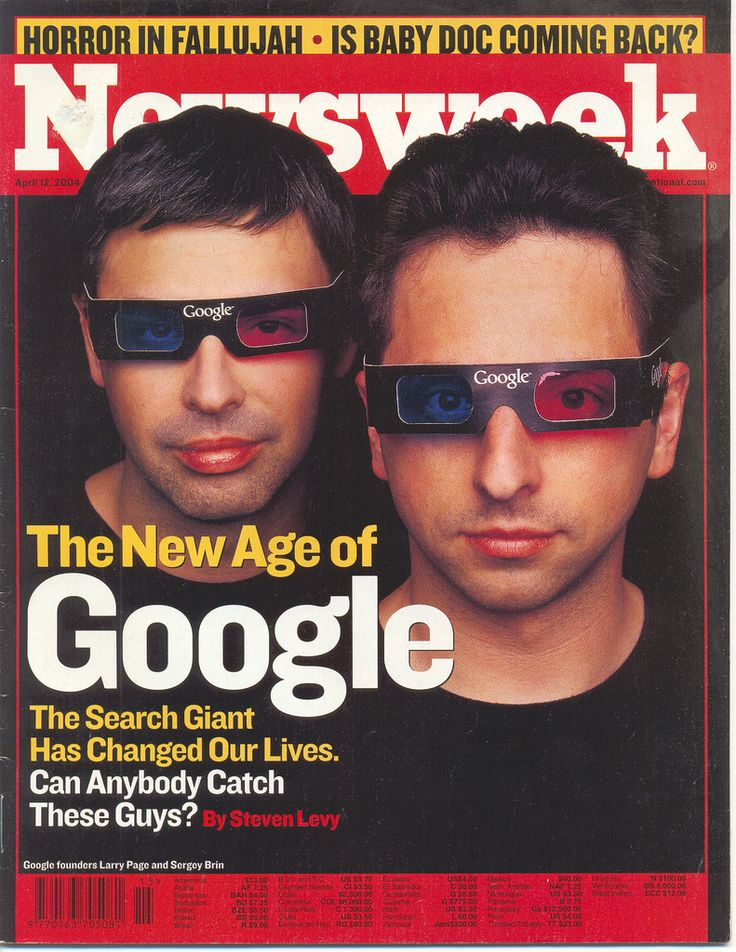
\includegraphics[width=1.\textwidth]{figs/extras/brin-page-newsweek1}

    .
    \column[T]{0.5\textwidth}
    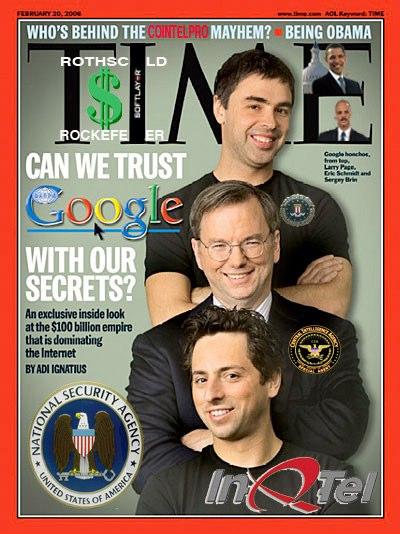
\includegraphics[width=1.\textwidth]{figs/extras/brin-page-time}
  \end{columns}
\end{frame}
%%%%%%%%%%%%%%%%%%%%%%%%%%%%%%%%%%%%%%%%
\begin{frame}{\PageRank : The model}{Measure of importance}
  \begin{columns}
    \begin{column}{0.3\textwidth}
      
\includegraphics[width=1.\textwidth]{figs/extras/penguin-no-spam}%{figs/extras/google-webspam}
    \end{column}
    \begin{column}{0.7\textwidth}

      % \structure{SP}iced h\structure{AM}

      \begin{exampleblock}{}%{Key}
        % While Google was not the first search engine, 
        % it was the first able to defeat the spammers who had made search almost useless.

        The \structure{importance} of a Web page is an inherently subjective matter...%, which depends on the readers interests, knowledge and attitudes. 
        But there is still much that can be said \alert{objectively} about the \structure{relative importance} of Web pages.

        \href{http://ilpubs.stanford.edu:8090/422/}{{\tiny
            \underline{Page, L.}; \underline{Brin, S.}; Motwani, R.; Winograd, T. (\underline{1999}) 
            \textit{The \textbf{PageRank} Citation Ranking: Bringing Order to the Web}. Tech.rep. \underline{Stanford} InfoLab.}}
      \end{exampleblock}
    \end{column}
  \end{columns}
  \pause
  \begin{centering}
    \structure{\fbox{Probability of visiting page by idealized random Web surfer}}
  \end{centering}
  \begin{block}{Why this trick works?}
    \begin{itemize}
    \item users of the Web ``vote with their feet'' %tend to place links to pages they think are good or useful
    \item users are more likely to visit useful pages
    \end{itemize}
  \end{block}
\end{frame}
%%%%%%%%%%%%%%%%%%%%%%%%%%%%%%%%%%%%%%%%
\begin{frame}{\PageRank : The model}{Random surfing as Markov process}
  % probability distribution for the location of a random surfer

  % \begin{block}{Hubbard model}
  \begin{columns}
    \column{0.2\textwidth}
    
\includegraphics[width=1.\textwidth]{figs/extras/web-surfer}
    \column{0.5\textwidth}
      \includegraphics<1>[width=1.\textwidth]{figs/tex/graph}
      \includegraphics<2>[width=1.\textwidth]{figs/tex/graph_probability0}
      \includegraphics<3>[width=1.\textwidth]{figs/tex/graph_probability1}
      \includegraphics<4>[width=1.\textwidth]{figs/tex/graph_probability2}
    \column{0.4\textwidth}
    
      \begin{exampleblock}{Probabilities}
        \begin{enumerate}
        \item<2-> $p = (1,0,0,0,0,0)$
        \item<3-> $p = (0,0,0,0,0,1)$
        \item<4-> $p = (0,\frac{2}{5},\frac{2}{5},\frac{1}{5},0)$
        \end{enumerate}
      \end{exampleblock}
  \end{columns}
  % \end{block}

   \pause
   \begin{block}{Restrictions}
     \begin{itemize}
     \item \structure{strongly connected} graph
     \item \structure{no dead-ends}
     \end{itemize}
   \end{block}
\end{frame}
%%%%%%%%%%%%%%%%%%%%%%%%%%%%%%%%%%%%%%%%
\begin{frame}{\PageRank : The model}{Transition matrix of the Web}
  % probability distribution for the location of a random surfer

  % \begin{block}{Hubbard model}
  \begin{columns}
    \begin{column}{0.45\textwidth}
      % 
\includegraphics[width=1.\textwidth]{figs/extras/term-spam-google}
    \end{column}
    \begin{column}{0.7\textwidth}

      \begin{exampleblock}{Restrictions}
        \begin{itemize}
        \item \structure{strongly connected} graph
        \item \structure{no dead-ends}
        \end{itemize}
      \end{exampleblock}
    \end{column}
  \end{columns}
  % \end{block}

   \pause
   \begin{block}{Restrictions}
     \begin{itemize}
     \item \structure{strongly connected} graph
     \item \structure{no dead-ends}
     \end{itemize}
   \end{block}
\end{frame}
%%%%%%%%%%%%%%%%%%%%%%%%%%%%%%%%%%%%%%%%
\begin{frame}{\PageRank : The model}{Structure of the Web}
  \begin{columns}
    \column{0.6\textwidth}
    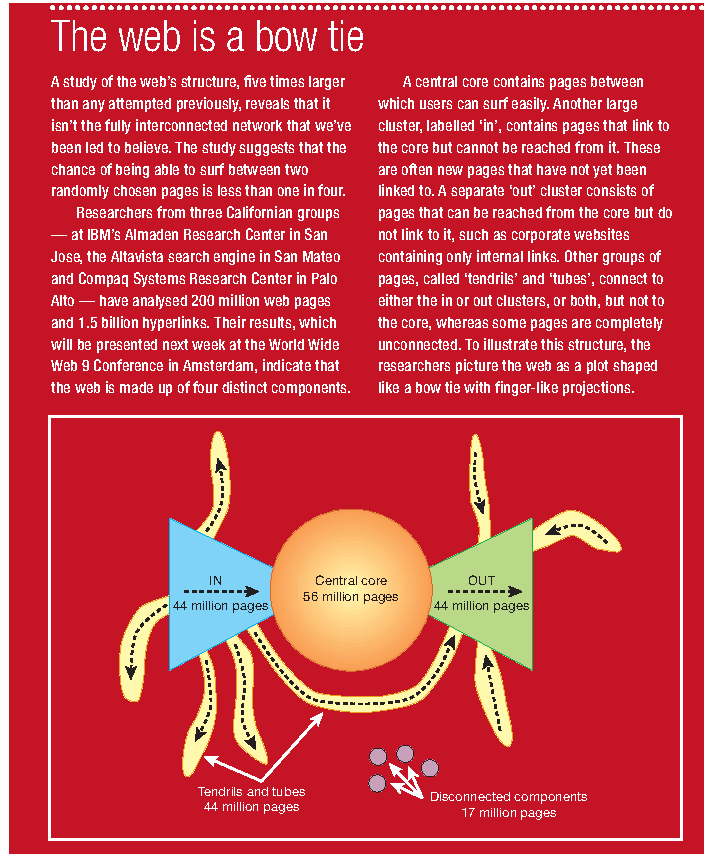
\includegraphics[width=1.\textwidth]{figs/pdf/BowTieExtract}%{WebBowTie}

    \column{0.4\textwidth}
    \href{http://www.nature.com/nature/journal/v405/n6783/pdf/405113a0.pdf}{\tiny \copyright \underline{\textit{Nature}} 405, 113 (11 May \underline{2000})}

    \begin{block}{Web as ``bowtie''}
      \begin{itemize}
      \item in-component
      \item out-component
      \item tendrils
        \begin{itemize}
        \item tubes
        \item isolated components
        \end{itemize}
      \end{itemize}
    \end{block}

    \pause
    \begin{block}{\alert{Problems}}
      \begin{itemize}
      \item \structure{dead-ends} %: no links out
      \item \structure{spider traps} %: have outlinks, but never link to any other pages
      \end{itemize}
    \end{block}
  \end{columns}
\end{frame}
%%%%%%%%%%%%%%%%%%%%%%%%%%%%%%%%%%%%%%%%
\begin{frame}{\PageRank : The model}{Avoiding dead ends by dropping}
  % A matrix whose column sums are at most 1 is called \structure{substochastic}
  \begin{columns}
    \column{0.5\textwidth}
    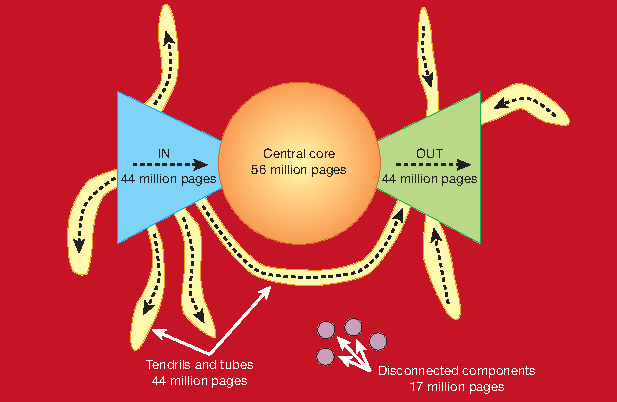
\includegraphics[width=1.\textwidth]{figs/pdf/WebBowTie}

    \column{0.5\textwidth}

    \begin{block}{Algorithm}
      \begin{enumerate}
      \item<1,2> \structure{Backward graph reduction}: remove dead ends iteratively
      \item<1,3> \structure{Compute {\PageRank}s} of reduced graph
      \item<1,4> \structure{Forward \PageRank computing}
      \end{enumerate}
    \end{block}
  \end{columns}
\end{frame}
%%%%%%%%%%%%%%%%%%%%%%%%%%%%%%%%%%%%%%%%
\begin{frame}{\PageRank : The model}{Teleporting}
  % A matrix whose column sums are at most 1 is called \structure{substochastic}
  \begin{columns}
    \column{0.5\textwidth}
    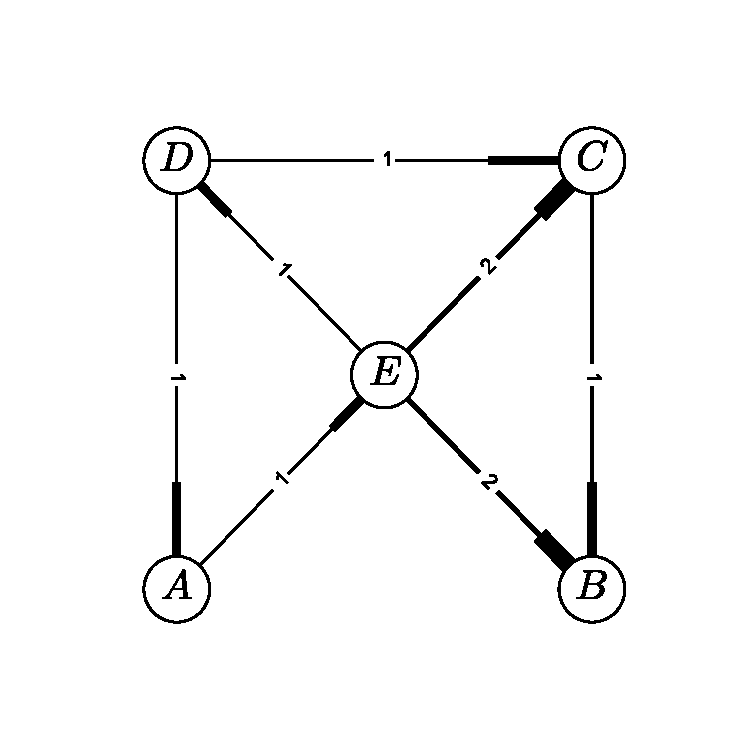
\includegraphics[width=1.\textwidth]{figs/tex/graph_dead_end}

    \column{0.5\textwidth}

    \begin{block}{Algorithm}
      \begin{enumerate}
      \item<1,2> \structure{Backward graph reduction}: remove dead ends iteratively
      \item<1,3> \structure{Compute {\PageRank}s} of reduced graph
      \item<1,4> \structure{Forward \PageRank computing}
      \end{enumerate}
    \end{block}
  \end{columns}

  \begin{equation*}
  \end{equation*}
\end{frame}
%%%%%%%%%%%%%%%%%%%%%%%%%%%%%%%%%%%%%%%%
\begin{frame}{Applications}{Major application areas}
  \begin{exampleblock}{Key}
    Yet the war between those who want to make the Web useful and those
    who would exploit it for their own purposes is never over.
  \end{exampleblock}

  \pause
  Techniques for preventing link spammers (search-engine optimization)
  \begin{itemize}
  \item TrustRank
  \item topic-sensitive \PageRank
  \end{itemize}
\end{frame}

\section{Algorithm}

\subsection{Serial BSOI algorithm}

\begin{frame}{Basic algorithms}{Framework}
  \begin{block}{Factorization-based approaches to matrix inversion}
    \begin{itemize}
    \item based on Gaussian elimination
      \begin{itemize}
      \item row partial pivoting is fast but unstable for $p$-cyclic matrices (S. Wright, 1993)
        %% \item panel rank-revealing pivoting strategy is stability in most cases but does not preserve structure
      \end{itemize}
    \item based on structured orthogonal factorization
      \begin{itemize}
      \item factorization is stable and has 
        identical complexity to the best known Gaussian elimination algorithms
      \end{itemize}
    \end{itemize}
  \end{block}

  \pause
  \begin{block}{Orthogonal inversion approach}
    \begin{centering}
      $\structure{\fbox{$H^{-1} = R^{-1}Q^T$}}$
    \end{centering}
    \begin{enumerate}
    \item Compute QR decomposition $H = QR$
    \item Invert the factor $R$ 
    \item Apply the factor $Q$ to $R^{-1}$ 
    \end{enumerate}
  \end{block}
\end{frame}

\begin{frame}{Basic algorithms}{Structured orthogonal factorization}
  \begin{block}{{\tt BSOF} -- Wright's serial version of SOF algorithm}
    \begin{algorithm}[H]%[thb]
      \KwData{$H$, $n$, $p$}
      \KwResult{$R$, $\{Q^{(k)} | 1 \leq k < p - 1 \}$}
      \BlankLine

      $R \gets O$; $\tilde{A}_1 \gets A_1$ ; $\tilde{B}_1 \gets B_p$\; 

      \For{$k \in \{1, 2,..., p-2 \}$ }{
        Compute regular QR: 
        $Q^{(k)} 
        \begin{bmatrix}
          R_{kk} \\ 0
        \end{bmatrix}
        =
        \begin{bmatrix}
          \tilde{A}_k \\ B_k
        \end{bmatrix}$\;

        %% Update 
        $\begin{bmatrix}
          R_{k,k+1} & R_{k,p} \\ \tilde{A}_{k + 1} & \tilde{B}_{k + 1}
        \end{bmatrix}
        \gets
        \left( Q^{(k)} \right)^{T} 
        \begin{bmatrix}
          0 & \tilde{B}_k \\ {A}_{k + 1} & 0
        \end{bmatrix}$;
      }
      
      Compute the QR: 
      $Q^{(p-1)} 
      \begin{bmatrix}
        R_{p-1,p-1} & R_{p-1,p}\\
        0 & R_{p,p}
      \end{bmatrix}
      = \begin{bmatrix}
        \tilde{A}_{p-1} & \tilde{B}_{p-1}\\ 
              {B}_{p-1} & {A}_{p,p}\\ 
      \end{bmatrix}$;
    \end{algorithm}
  \end{block}
\end{frame}

\begin{frame}{Basic algorithms}{Inversion via block back substitution}
  \begin{block}{{\tt BSTRI\_RV} -- Row Version of the BBS}
    \begin{algorithm}[H]
      \SetKwFunction{Batched}{Batched}

      \KwData{$R$, $n$, $p$}
      \KwResult{$X$}
      \BlankLine

      $X \gets O$\; 
      $X_{p-2:p,p-2:p}\gets R_{p-2:p,p-2:p}^{-1}$\;
      \Batched$_{i = 1:p-3}$ \{$X_{ii}\gets R_{ii}^{-1}$\} \;
      $X_{1:p-3,p}\gets R_{1:p-3,p} X_{p,p} $ \;
      \Batched$_{i = 1:p-3}$ \{$X_{i,p}\gets -X_{ii}  R_{i,p}$, $X_{i,i+1}\gets -X_{ii}  R_{i,i+1}$ \} \;
      \For{$i \in \{p-3, p-4,..., 1 \}$ }{ 
        $X_{i,i+2:p} \gets X_{i,i+2:p} + X_{i,i+1} X_{i+1,i+2:p} $ \;  
        $X_{i,i+1} \gets X_{i,i+1}  X_{i+1,i+1}$\;}
    \end{algorithm}    
  \end{block}
  
  \begin{block}{{\tt BSTRI\_CV} -- Column Version of the BBS}
    Similar to {\tt BSTRI\_RV}
  \end{block}
\end{frame}

\begin{frame}{Basic algorithms}{Complexity}  
  \begin{block}{Operation counts}
    \begin{center}
      \rowcolors[]{1}{blue!20}{blue!10} %\rowcolors{1}{Blue!20}{Blue!5}
      \begin{tabular}{r|l|c|c|c}
        \toprule
        Phase & Routine & Additions & Multiplications & Total Flops  \\
        \hline
        I&{\tt BSOF} & 
        $\displaystyle\Theta\left(\frac{23}{3} n^{3} p\right)$
        & $\displaystyle\Theta\left(\frac{23}{3} n^{3} p\right)$
        & $\displaystyle\Theta\left(\frac{46}{3} n^{3} p\right)$\\
        II&{\tt BSTRI\_RV} & 
        $\displaystyle\Theta\left(\frac{1}{2} n^3 p^{2}\right)$
        & $\displaystyle\Theta\left(\frac{1}{2} n^3 p^{2}\right)$
        & $\displaystyle\Theta\left(n^3 p^{2}\right)$\\
        \cline{2-5}
        &{\tt BSTRI\_CV} & 
        $\displaystyle\Theta\left(n^3 p^{2}\right)$
        & $\displaystyle\Theta \left(n^3 p^{2}\right)$
        & $\displaystyle\Theta \left(2 n^3 p^{2}\right)$\\
        III&{\tt BSOI} & 
        $\displaystyle\Theta \left(3 n^3 p^2\right)$
        & $\displaystyle\Theta \left(3 n^3 p^2\right)$
        & $\displaystyle\Theta \left(6 n^3 p^2\right)$\\
        \bottomrule  
      \end{tabular}
    \end{center}
    \pause
    To sum up, 
    \[
    \fbox{
      $\text{Total complexity} = \alert{\displaystyle\Theta\left(\frac{7}{2} n  N^2\right)}$}
    \]
  \end{block}
\end{frame}


\section{Experimental results and analysis}

\begin{frame}{Experimental results}{Experimental setup}
  \renewcommand*\DTstyle{\sffamily\small}
  \renewcommand*\DTstylecomment{\footnotesize\textsl}
  \DTsetlength{0.2em}{1em}{0.2em}{0.4pt}{0.4pt}
  \begin{itemize}
  \item \structure{Hardware}
    \begin{columns}
      \begin{column}{.5\textwidth}
        \dirtree{%
          .1 \structure{Single-GPU}\DTcomment{Hybrid node at UCD}.
          .2 2 $\times$ Intel Xeon X5670.
          .3 6-cores, 2.9GHz.
          .2 1 $\times$ %% CUDA-enabled
          NVIDIA GTX480. %, Fermi
          .3 15 SMs $\times$ 32 cores.
        }
      \end{column}
      \begin{column}{.5\textwidth}
        \dirtree{%
          .1 \structure{Multi-GPU}\DTcomment{Dirac cluster at NERSC}.
          .2 2 $\times$ Intel Xeon E5530. %Nehalem
          .3 4-cores, 2.4 GHz.
          .2 4 $\times$ NVIDIA Tesla C1060.
          .3 240 cores. %1.296 GHz
        }
      \end{column}
    \end{columns}

  \item \structure{Software}
    \begin{itemize}
    \item POSIX threads for threading in step 2 of \Bsoftri
    \item CuBlas, Magma, and Intel's MKL for LAPACK interface
    \end{itemize}
    
  \item \structure{Codes}
    \begin{itemize}
    \item stand-alone CPU, stand-alone GPU, and hybrid CPU+GPU implementations
    \item publicly available at
      \url{https://github.com/SGo-Go/BSOFI}
    \end{itemize}
  \end{itemize}
\end{frame}

\begin{frame}{Experimental results}{Performance tuning}

  \begin{block}{Performance tuning approach}
    benchmark LAPACK kernels 
    $\to$
    approximate parameters of PM %performance model
    $\to$
    embed approximates into the code
  \end{block}

  \begin{columns}<2->[t]%[thb]
    \begin{column}[t]{0.5\textwidth}
      \centering
      CPU/GPU performance ratio parameters 
      ($\kappa_R$, $\kappa_C$, and $\kappa_Q$)

      % \visible<2->{
      % 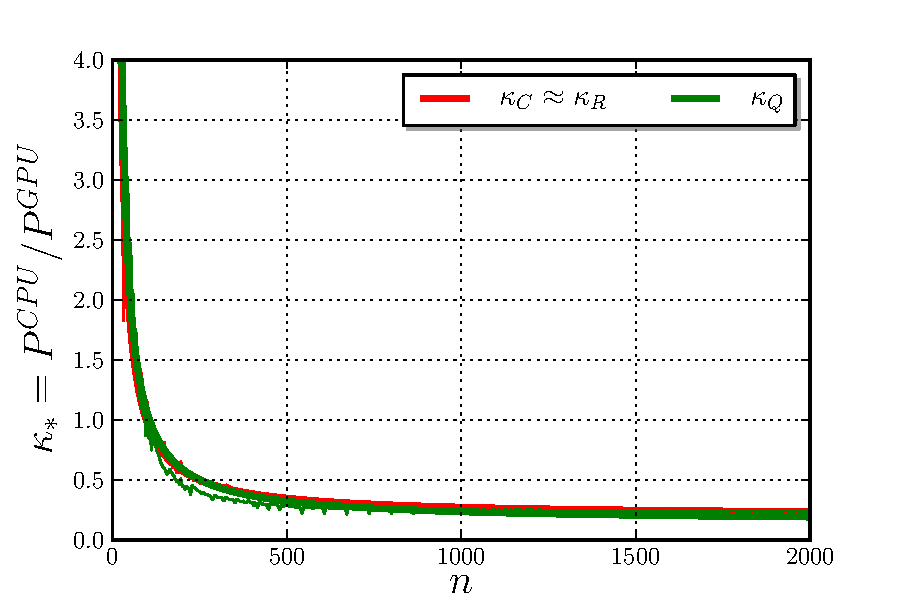
\includegraphics[width=\textwidth]{./figs/pdf/kappa_params}}
      
      %% Approximation approach
      \begin{itemize}
        \small
      \item 1st order rational functions of $n$
      \item Gauss-Markov estimator
      \end{itemize}
    \end{column}

    \begin{column}[t]{0.5\textwidth}
      \centering
      Switching ($l_F$) and  correction parameters 
      ($c_i$, $c_j$, $c'_k$, and $c''_k$)
      % \visible<2->{
      %   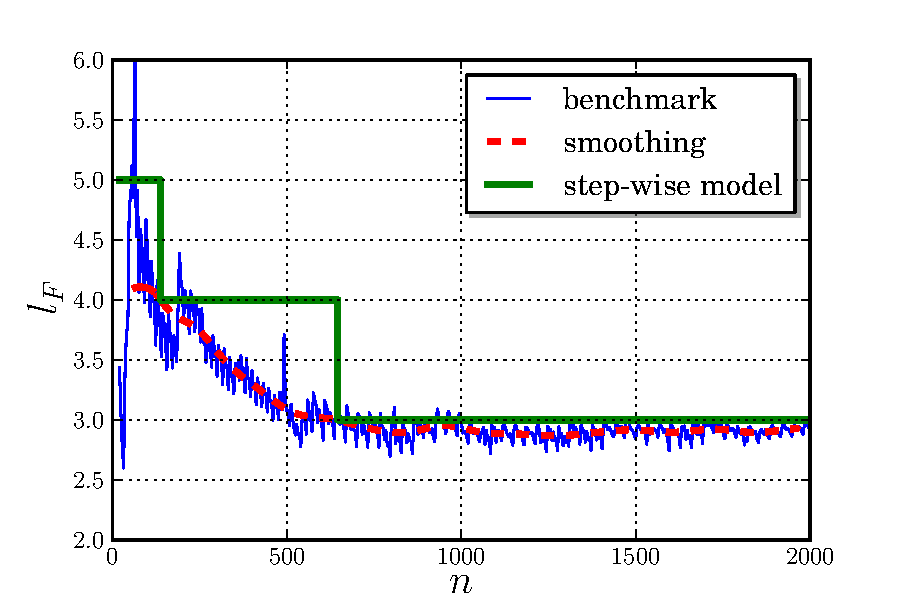
\includegraphics[width=\textwidth]{./figs/pdf/lF_param_approx}}

      %% Approximation approach
      \begin{itemize}
        \small
      \item %% descending 
        step-wise functions of $n$
      \item 1D filtering + rounding
      \end{itemize}
    \end{column}

  \end{columns}
\end{frame}

%% \frame[plain]{\centering
%%   \Huge Thank you for your attantion!
%%   \includegraphics[height=0.5\textheight]{figs/extras/question.jpg}
%% }

\end{document}
